\documentclass[8pt]{article}
\usepackage[utf8]{inputenc}
%\usepackage{fullpage}
\usepackage[portuguese]{babel}
\usepackage{amssymb}
\usepackage{multicol}
\usepackage{graphicx}
\usepackage{multicol}
\usepackage{wrapfig} % para colocar figura flutuando ao lado do texto
\usepackage{caption} % para retirar caption de figura
\usepackage{subcaption} % para colocar figuras lado a lado

\renewcommand{\emph}[1]{\textbf{#1}}

%\newcommand{\mycell}[3]{ #1 & #2 & \parbox{12cm}{#3} \\ \hline }
\newcommand{\mycell}[3]{

  #1 & #2 & \parbox{6cm}{
    \vspace{.1\baselineskip}
    #3
    \vspace{.1\baselineskip}
  } \\ \hline
}
\newcommand{\titulo}[1]{{\bf #1}}

\newcommand{\itspc}{
  \vspace{-8pt}
  \setlength\itemsep{-4pt}
}

\begin{document}

\pagenumbering{gobble}

\begin{center}
{\Large \bf Segundo Trabalho de Elementos de Lógica Digital - 2015/2}
\\
23/10/2015
\vspace{5mm}
\end{center}

\noindent
\titulo{Professor:} Marcos Daniel Baroni $<$\texttt{marcos.baroni@aluno.ufes.br}$>$

\noindent
\titulo{Data de entrega:} 12 de novembro de 2015

\noindent
\titulo{Regras:}
\begin{enumerate}
  \item O trabalho será feito sozinho ou em dupla;
  \item Não será tolerado plágio;
  \item Utilizar o Logisim (\texttt{http://www.cburch.com/logisim/}) e o arquivo
    \texttt{trab2.circ} que foi enviado.
  \item \underline{Trabalhos fora de padrão serão penalizados.}
\end{enumerate}


\noindent
\titulo{Material a ser entregue:}
\begin{enumerate}
  \item{Arquivo de simulação ``\texttt{trab2.circ}'' contendo os devidos circuitos:}
  \begin{itemize}
	\item{Enviar por email para \texttt{marcos.baroni@aluno.ufes.br} contendo os devidos circuitos;}
	\item{O título do email deve ser \texttt{"ELD:TRAB2:nome1:nome2"} \\ { Ex.: \texttt{"ELD:TRAB2:alanturing:donaldknuth"}};}
	\item{Os circuitos devem estar separados em blocos, conforme enunciado. }
  \end{itemize}
  \item{Relatório:}
  \begin{itemize}
	\item{Deverá ser entregue \underline{em formato PDF}, enviado por email, juntamente do arquivo ``trab2.circ''.}
    \item{O relatório deve conter explicações dos passos realizados.}
  \end{itemize}
\end{enumerate}

\noindent
\titulo{Orientações para utilização do Logisim:}
\begin{itemize}
  \item Para testar os circuitos, sugiro utilizar o tipo ``Botão'' como clock.
  \item Para criar um novo circuito:
  \begin{enumerate}
    \item No painel lateral, clique com o botão direito do mouse em "trab2";
    \item Selecione ``Acrescentar circuito...''.
  \end{enumerate}
  \item Para adicionar um bloco ao circuito:
  \begin{enumerate}
    \item No painel lateral, clique com o mouse sobre o circuito ao qual deseja-se utilizar como bloco e arraste-o para a área de montagem.
  \end{enumerate}
\end{itemize}

\newpage
\noindent
\titulo{\large Simulação 1: Conversão de dado paralelo-série} \\
Construir um conversor de dado ``paralelo-série'' e um conversor ``série-paralelo'',
para dados de 4 bits.
O conversor ``paralelo-série'' deve possuir uma porta ``Enable'' que ao ser ligada habilita a escrita do dado em paralelo.
Para fins de organização deverão ser criados (ao menos) 2 circuitos auxiliares, um circuito para cada conversor.
A Figura~\ref{fig:sim1} apresenta um esboço desta simulação, que deverá ser montada no circuito ``Simulação 1''.

\begin{figure}[h]
  \centering
  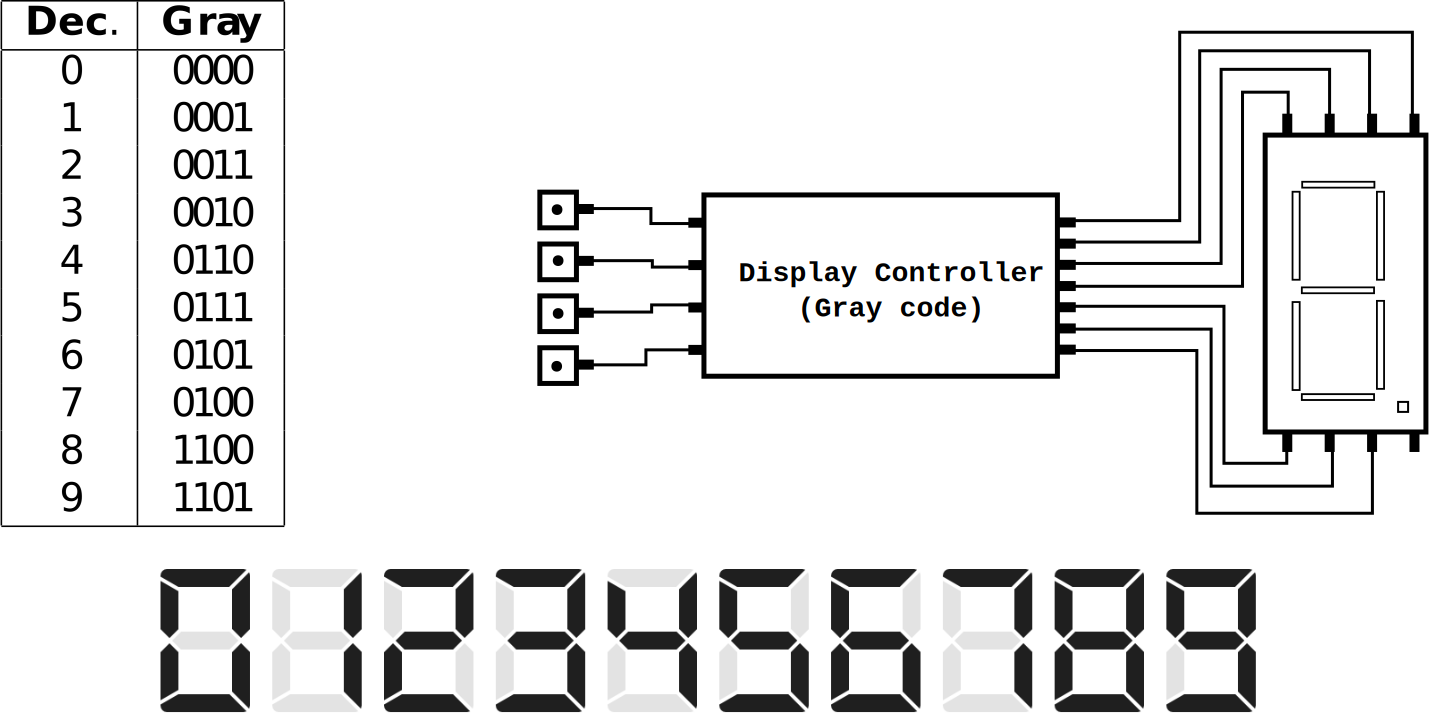
\includegraphics[scale=0.3]{figs/sim1}
  \caption{Esboço da Simulação 1.}
  \label{fig:sim1}
\end{figure}

\vspace{3mm}
\noindent
\titulo{\large Simulação 2: Contador de sequência qualquer} \\
\noindent
Construir um contador síncrono que conte a sequência apresentada na Figura~\ref{fig:seq}.
O contador deve possuir uma entrada ``Clear'' que reinicia o contador imediatamente (coloca-o em $0$).
Para fins de organização deverá ser criado (ao menos) 1 circuito auxiliar, contendo o contador.
Para testar o funcionamento do circuito, utilize o display de 7 segmentos e o bloco ``controle-display'' já existente no arquivo.
A Figura~\ref{fig:sim2} apresenta um esboço desta simulação, que deverá ser montada no circuito {``Simulação~2''}.

\begin{figure}[h]
  \centering
  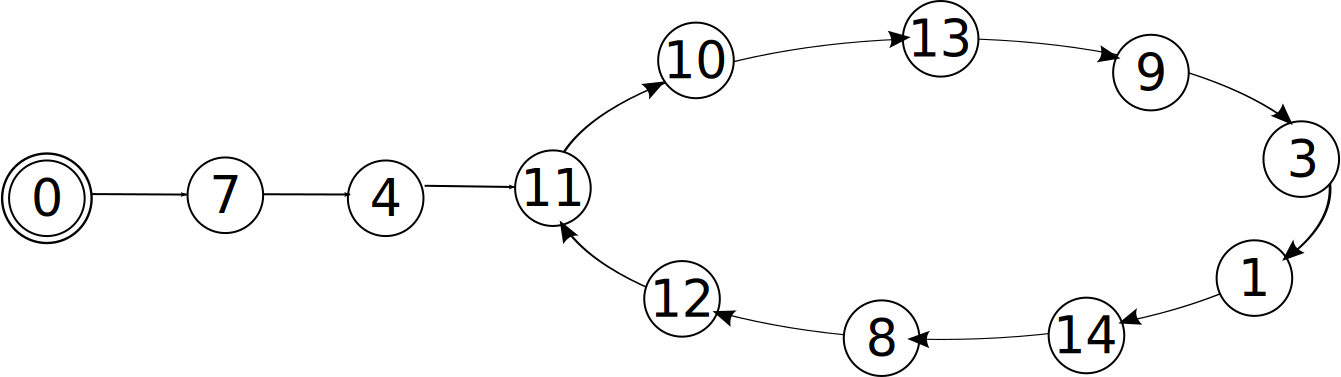
\includegraphics[scale=0.28]{figs/seq_b}
  \caption{Sequência a ser contada.}
  \label{fig:seq}
\end{figure}

\begin{figure}[h]
  \centering
  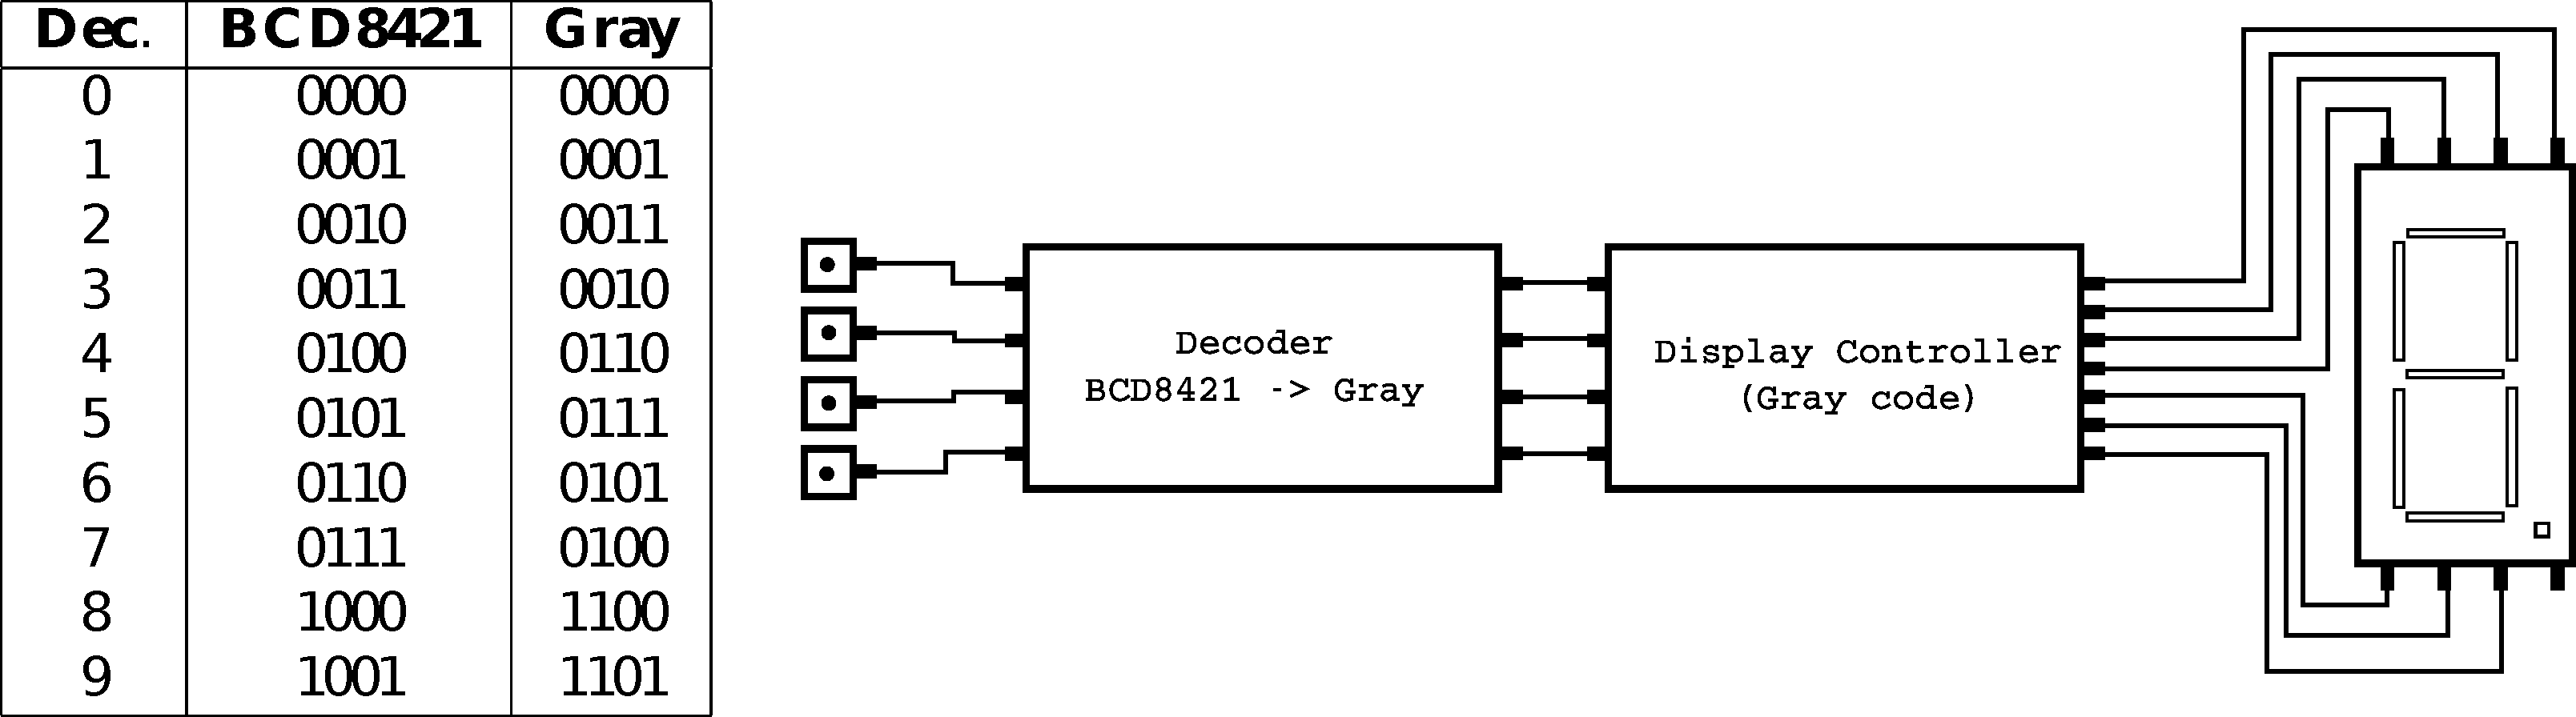
\includegraphics[scale=0.4]{figs/sim2}
  \caption{Esboço da Simulação 2.}
  \label{fig:sim2}
\end{figure}

%\vspace{-18mm}
%\begin{figure}
%\begin{minipage}{.5\textwidth}
%  \centering
%  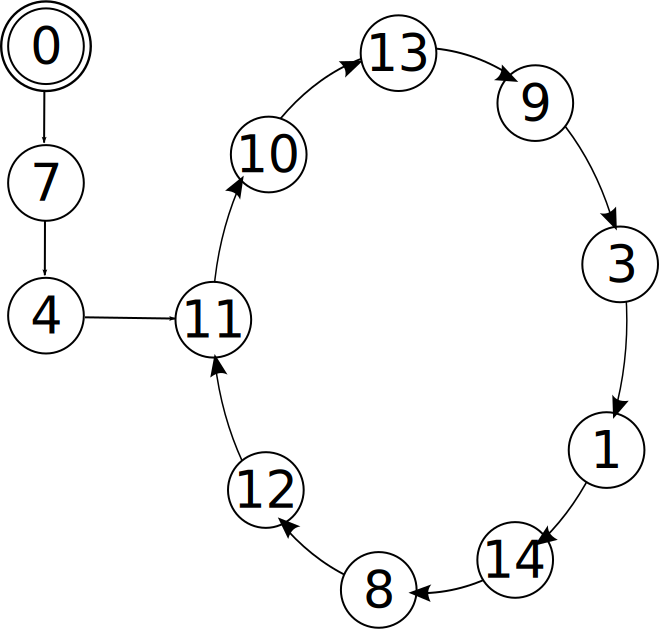
\includegraphics[scale=0.28]{figs/seq}
%  \caption{Sequência a ser contada.}
%  \label{fig:seq}
%\end{minipage}%
%\begin{minipage}{.5\textwidth}
%  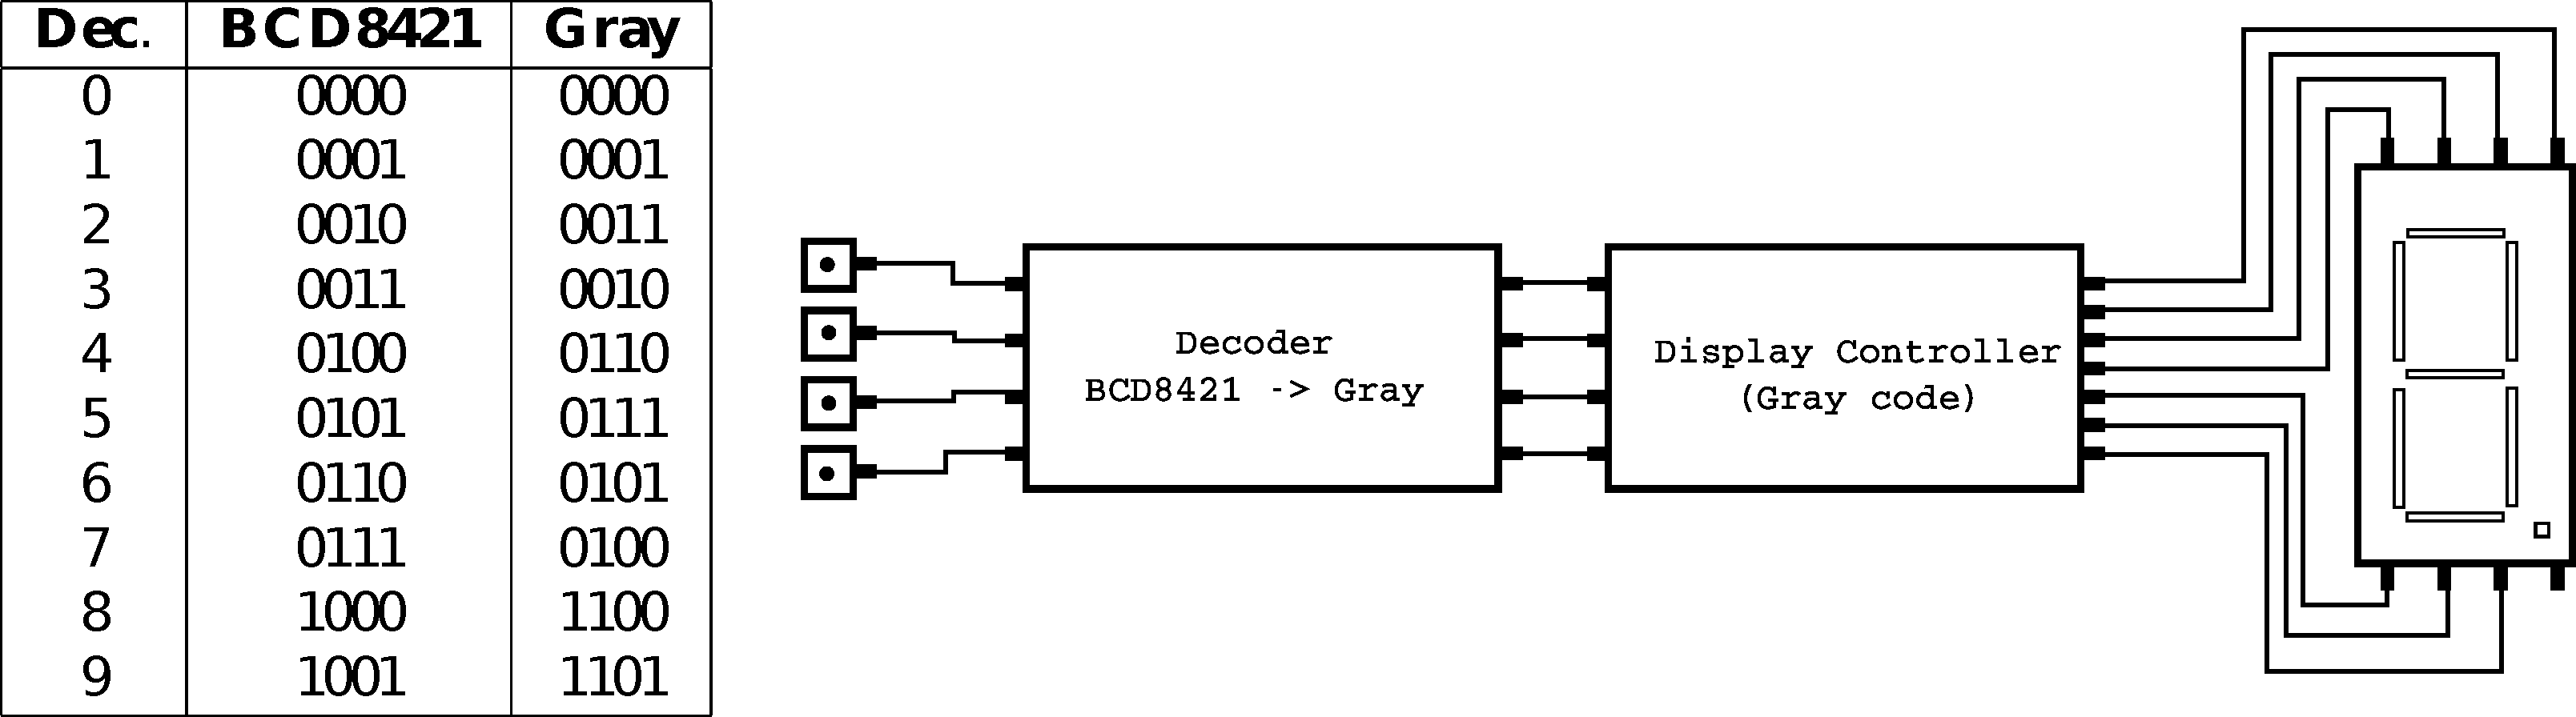
\includegraphics[scale=0.6]{figs/sim2}
%  \caption{Esboço da simulação 2.}
%  \label{fig:sim2}
%\end{minipage}
%\end{figure}

\end{document}

